% UQ Gemini theme
% See: https://github.com/alfurka/gemini-uq
% Forked from
% https://rev.cs.uchicago.edu/k4rtik/gemini-uccs
% which is forked from
% https://github.com/anishathalye/gemini


\documentclass[final]{beamer}

% ====================
% Packages
% ====================

\usepackage[T1]{fontenc}
\usepackage{xcolor}
\usepackage{lmodern}
\usepackage[size=custom,width=100,height=75,scale=1.0]{beamerposter}
\usetheme{gemini}
\usecolortheme{gemini}
\usepackage{graphicx}
\usepackage{booktabs}
\usepackage{tikz}
\usepackage{pgfplots}
\pgfplotsset{compat=1.17}

% ====================
% Lengths
% ====================

% If you have N columns, choose \sepwidth and \colwidth such that
% (N+1)*\sepwidth + N*\colwidth = \paperwidth
\newlength{\sepwidth}
\newlength{\colwidth}
\setlength{\sepwidth}{0.025\paperwidth}
\setlength{\colwidth}{0.3\paperwidth}

\newcommand{\separatorcolumn}{\begin{column}{\sepwidth}\end{column}}


% ====================
% Title
% ====================

\title{Running a Carpentries Workshop without the Internet}

\author{Jannetta S. Steyn \inst{1} \and Colin Sauze \inst{2} \and Abhishek Dasgupta \inst{3}}

\institute[shortinst]{\inst{1} Newcastle University \samelineand \inst{2}National Oceanography Centre \samelineand \inst{3} University of Oxford} 

% ====================
% Footer (optional)
% ====================

\footercontent{
	\href{https://carpentriesoffline.org}{https://carpentriesoffline.org} \hfill
	RSECon 2023 - Swansea \hfill
	\href{mailto:jannetta.steyn@newcastle.ac.uk}{jannetta.steyn@newcastle.ac.uk}
}
% (can be left out to remove footer)

% ====================
% Logo (optional)
% ====================

% use this to include logos on the left and/or right side of the header:
% \logoright{\includegraphics[height=7cm]{logo1.pdf}}
% \logoleft{\includegraphics[height=7cm]{logo2.pdf}}

% ====================
% Body
% ====================

\begin{document}
	\addtobeamertemplate{headline}{}
	{
		\begin{tikzpicture}[remember picture,overlay]
			\node [anchor=north west, inner sep=3cm] at ([xshift=-0.5cm,yshift=0.5cm]current page.north west)
			{
\includegraphics[height=4.5cm]{logos/OFFLINE.png}}; % also try shield-white.eps
			\node [anchor=north east, inner sep=3cm] at ([xshift=0.0cm,yshift=2.5cm]current page.north east)
			{
\includegraphics[height=8.0cm]{logos/qr.png}};
		\end{tikzpicture}
	}
	
	\begin{frame}[t]
		\begin{block}{\large Abstract}	

			CarpentriesOffline (https://carpentriesoffline.org) is an out of the box solution for running a Carpentries workshop from a single device such as a Raspberry Pi (RPi), old laptop or even a dedicated server. It is intended for use in environments where there is limited or no internet access. Everything needed to run the workshop including course notes, data files, software downloads, a Git server, etherpad and a JupyterHub server are provided by the CarpentriesOffline system. It can also provide a backup environment for those with better connectivity in the event of the Carpentries website, etherpad, GitHub etc suffering an outage.
		\end{block}
	
		\begin{columns}[t]
			\separatorcolumn
			
			
			\begin{column}{\colwidth}
				
				\begin{block}{Raspberry Pi Solution}
					\begin{center}
						\begin{figure}
							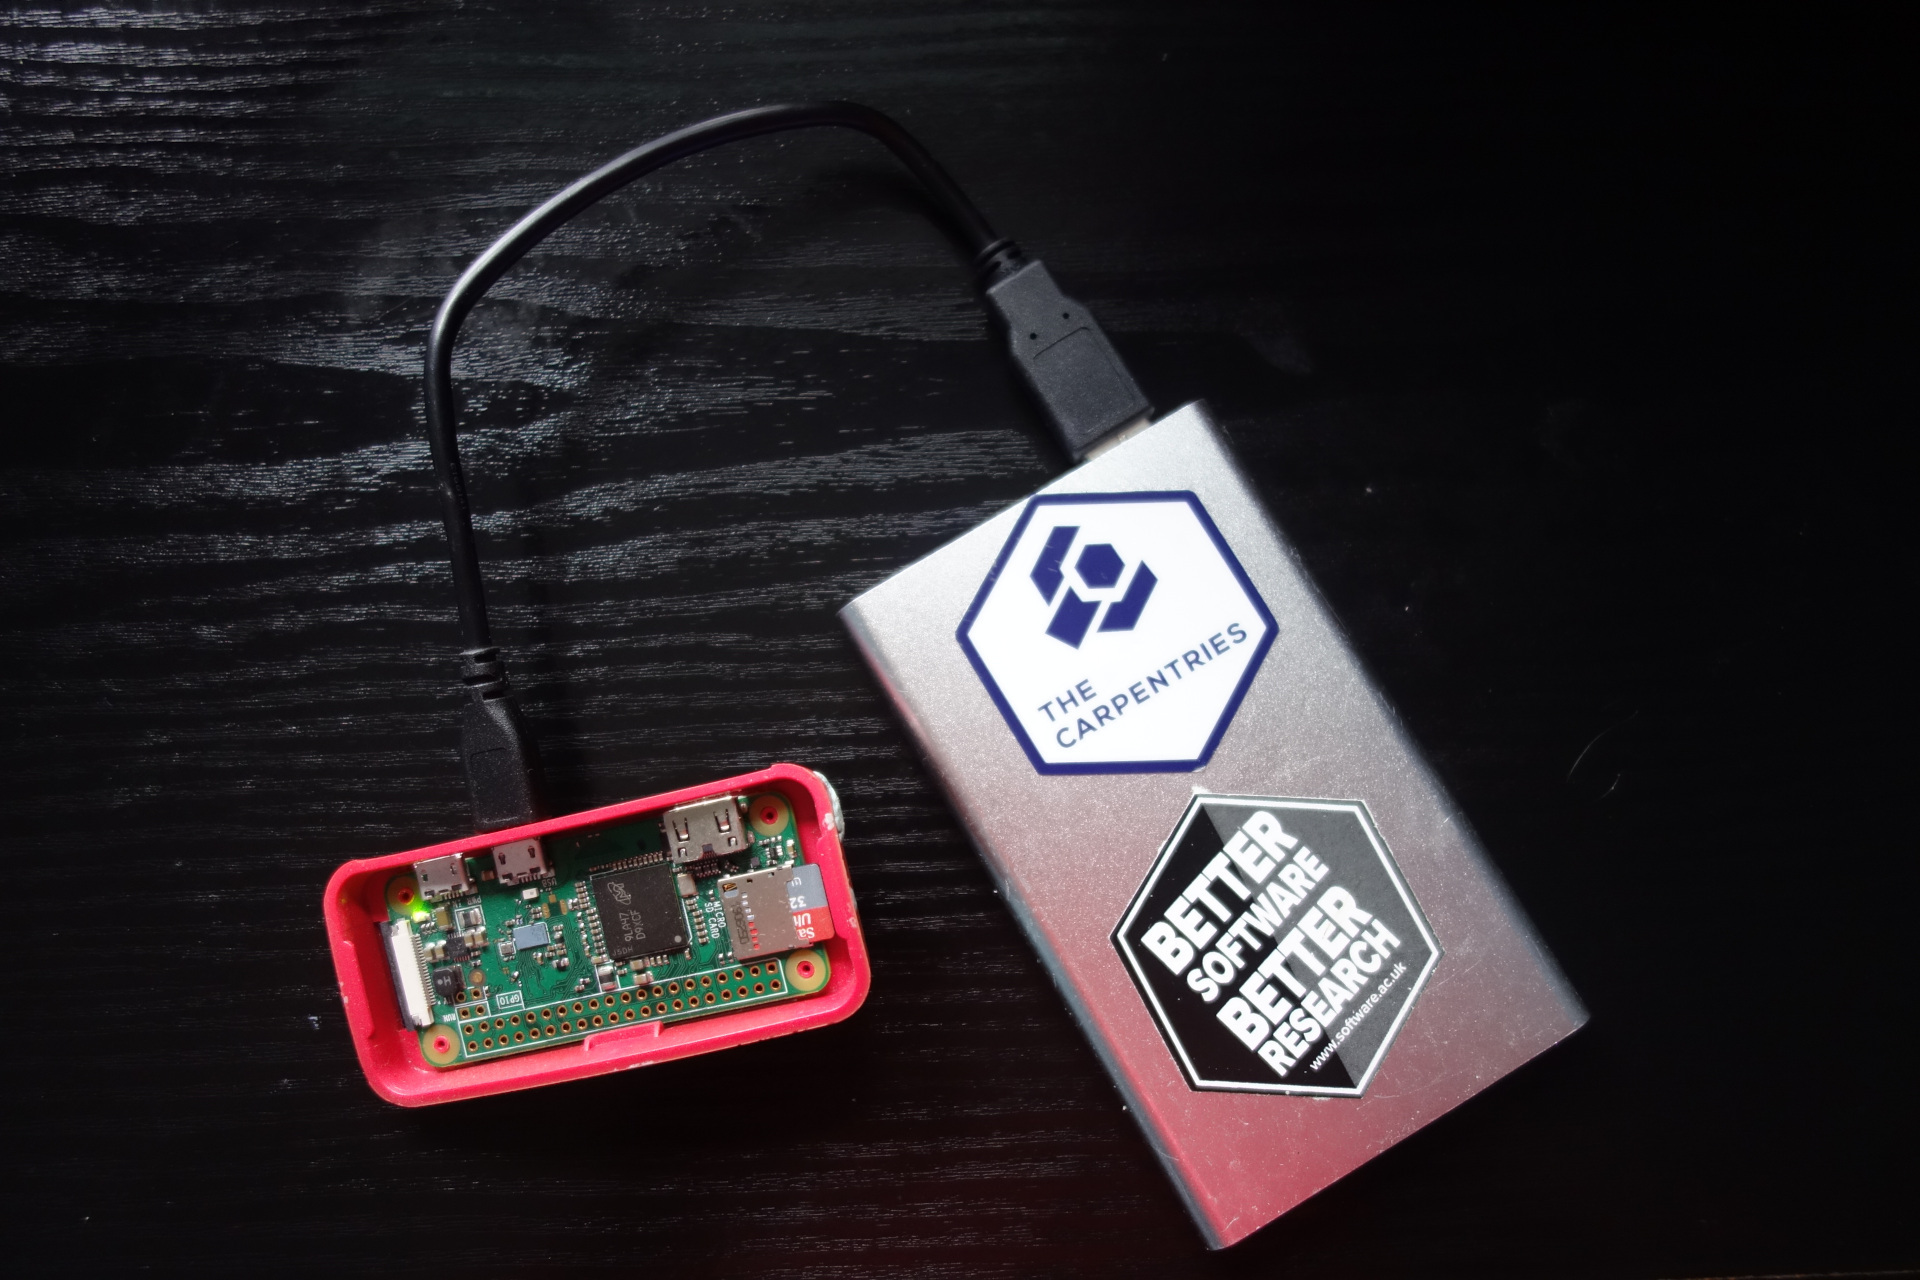
\includegraphics[width=0.6\columnwidth]{logos/CarpentriesOfflinePhoto.png}
							\caption{A Raspberry Pi Zero running CarpentriesOffline on RPi OS and powered with a USB Power Bank - tested at RSECon2022}
						\end{figure}
					\end{center}

					
				\end{block}
				
				\begin{alertblock}{Carpentries in your Pocket}
					
					RPis are credit card sized computers that are used in education and by hobbyists to learn about computing and electronics. 
					These little computers have many applications including being used as workstations and servers. For CarpentriesOffline we turn a single 
					Raspberry Pi into a WiFi access point as well as a web server that serves Carpentries lessons, offers all the downloads required for 
					learners to install on their computers as well as Gitea which is a replacement service for GitHub. An image that can be written to 
					a microSD card is available for download. Once the image is written to the microSD card it can be inserted into the RPi and with no 
					further effort the RPi should boot into a server offering all the above mentioned services.					
				\end{alertblock}
				
				\begin{block}{Server Software for CarpentriesOffline}
					\begin{table}
						\caption{Pebble the RockPi version}				
						\begin{tabular}{l}
							\textbf{Item} \\
							\hline
							Apache Web Server \\
							Gitea \\
							MiniCRAN \\
							Carpentries Lessons \\
							Software downloads \\
						\end{tabular}
					\end{table}
				\end{block}
			\end{column}
			
			\separatorcolumn
			
			\begin{column}{\colwidth}
				
				\begin{block}{FlashDrive Solution}
					\begin{figure}
						\begin{center}
							\includegraphics[width=0.6\columnwidth]{logos/FlashDrive.png}
							\caption{A bootable flashdrive with Debian based Slax Linux and everything needed to turn a laptop into an access point and a web server}
						\end{center}
					\end{figure}
				\end{block}
			
				\begin{alertblock}{Carpentries on a Stick}			
					RPis are relatively cheap but in communities where Internet access is problematic it is likely that they are either not available or still 
					costly. Most researchers will already have either a laptop of their own or one provided by their institution. Most laptops can boot from 
					a USB device such as a flashdrive. As with the microSD card image for the RPi we have created an image that can be written to a flashdrive 
					and allows the computer to boot into a Linux distro (Debian based Slax) which turns the computer into a server with the same functionality 
					provided on the microSD card. For the moment we only have an image for PCs, but we are looking into creating an option for Macs.
				\end{alertblock}
			
				\begin{block}{CarpentriesOffline Home Page}
					\begin{figure}
						\begin{center}
							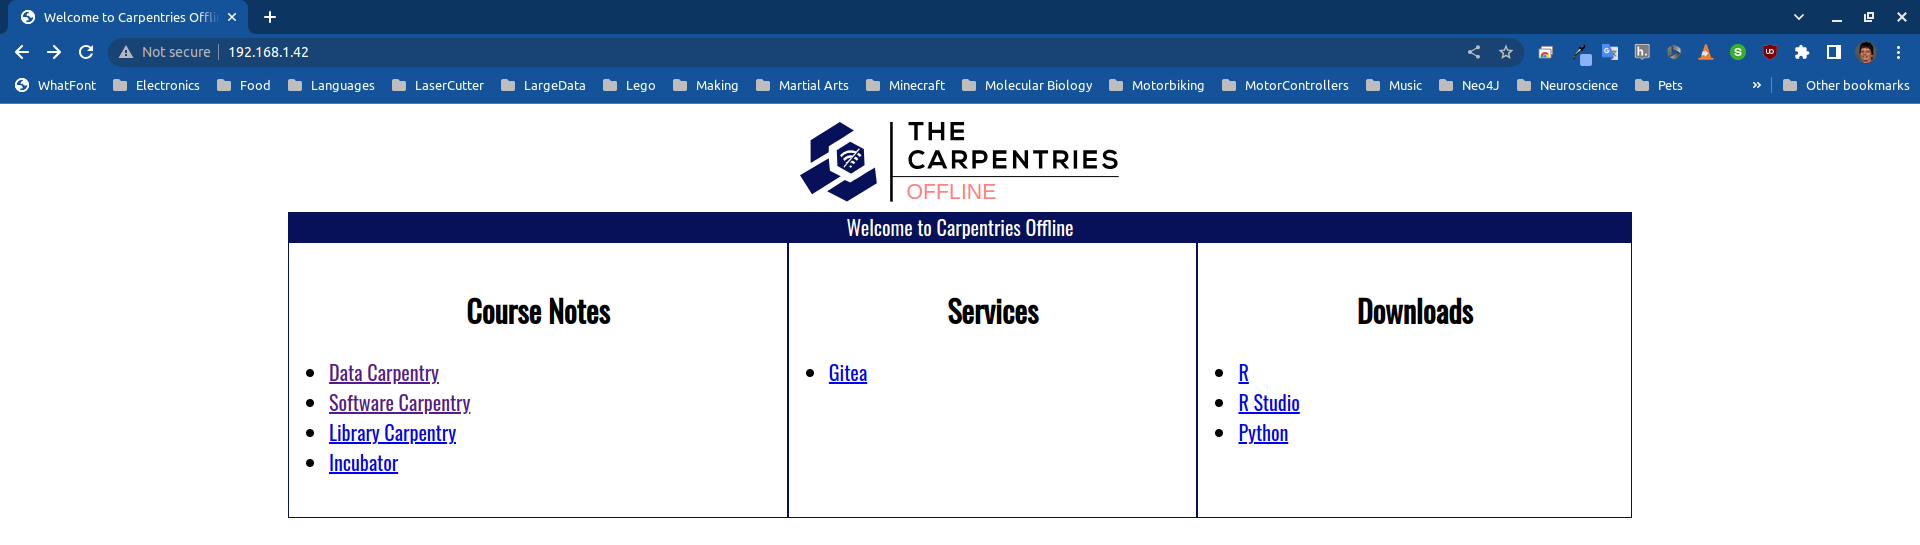
\includegraphics[width=0.9\columnwidth]{logos/webpage.png}
							\caption{The CarpentriesOffline Home Page allows learners to download everything they need as well as provide Gitea to replace GitHub.}
						\end{center}
					\end{figure}
				\end{block}

			\end{column}
			
			\separatorcolumn
			
			\begin{column}{\colwidth}
				
				\begin{block}{The miniHPC }

					\begin{figure}
						\begin{center}
							\includegraphics[width=0.9\columnwidth]{logos/mini-HPC-proto1.png}
							\caption{Pixie the prototype miniHPC built from RPi4s using pre-owned RPi 4s. 
								For the next iteration we bought Rock Pi 4C+}
						\end{center}
					\end{figure}
				\end{block}

				\begin{alertblock}{Why?}
					Why build yet another miniHPC? There are quite a few around already. However, none of these 
					are aimed at continuous use in training and prototyping. We aim to provide detailed instructions
					for building a miniHPC but then also Carpentries style lessons for instructors to use these 
					miniHPCs in workshops. The advantages are many:
					
					\begin{itemize}
						\item \textbf{More control} over the hardware.
						\item \textbf{Obtaining user accounts} on HPCs can be difficult and often
						learners do not register in time.
						\item \textbf{Avoids extra load} on a real HPC that is being used for research.
						\item \textbf{Visible hardware} makes the concept of an HPC less abstract to learners.
						\item \textbf{Resource limits} are more apparent. 
					\end{itemize}
				\end{alertblock}		
					
				\begin{block}{Bills of Material}
					\begin{table}
%						\parbox{.45\linewidth}{
%							\centering
%							\caption{Pixie the Prototype}			
%							\begin{tabular}{l c}
%								\textbf{Item} & \textbf{Qty} \\
%								\hline
%								Raspberry Pi 4 & 5 \\
%								Power supply & 5 \\
%								8 port switch & 1 \\
%								8 port strip plug & 1 \\
%								Short Cat 6 10baseT & 8 \\
%								Cooling fan & 1 \\
%								DIN Rail & 1 \\
%								3D printed rail stand & 2 \\
%								3D printed DIN rail cases & 5 \\
%								 & \\
%							\end{tabular}
%						}
%						\hfill
						\parbox{.45\linewidth}{
							\centering
							\caption{Pebble the RockPi version}				
							\begin{tabular}{l c}
								\textbf{Item} & \textbf{Qty} \\
								\hline
								RockPi 4C+ & 8 \\
								RockPi 4SE & 1 \\
								Power supply & 1 \\
								10 port switch & 1 \\
								4 port strip plug & 1 \\
								Short Cat 6 10baseT & 9 \\
								Dual Cooling fan & 1 \\
								DIN Rail & 1 \\
								3D printed rail stand & 2 \\
								3D printed DIN rail cases & 9 \\
							\end{tabular}
						}
						\parbox{.45\linewidth}{
							\centering
							\caption{Software}				
							\begin{tabular}{l|l}
								\textbf{Product} & {Purpose}\\
								\hline
								Slurm & Job Scheduler \\
								lmod & Module System \\
								MPICH & HPC MPI \\
								Ansible & Deployment \\
								PXE & Boot over Network \\
								NFS & Network File System \\
								Munge & Authentication \\
								DHCP & IP Allocation \\
								EasyBuild & Software Building \\
							\end{tabular}
						}
					\end{table}
				\end{block}	
			\end{column}			
			\separatorcolumn
		\end{columns}
	\end{frame}
	
\end{document}
